% BEGIN PREAMBEL
\documentclass[9pt]{beamer}
\usepackage[british]{babel}
\usepackage[latin1]{inputenc}
\usepackage{multimedia}
\usepackage{amsmath,amsfonts,amssymb}
\usepackage{upgreek}
\usepackage{pgfpages}
\usepackage[version=3]{mhchem}
\usepackage{lmodern}
\usepackage{graphicx}
\usepackage{multicol}
\usepackage{color}
\usepackage{xcolor,fontawesome}
\usepackage{wrapfig}
\usepackage{siunitx}
\usepackage{fontspec}
\usepackage{tikz}
\usepackage{textpos}
\usepackage{booktabs}
\newfontfamily\ubuntu{Ubuntu}
\newcommand{\as}{\\[14pt]}
\newcommand{\s}{\\[7pt]}
\newcommand{\is}{\\[2pt]}
\newcommand{\no}{\noindent}
\newcommand{\ka}{\hspace*{0.5cm}}
\newcommand{\ma}{\hspace*{1cm}}
\newcommand{\ga}{\hspace*{1.5cm}}
\newcommand{\li}{\left|}
\newcommand{\re}{\right|}
\newcommand{\const}{\text{const.}}
\newcommand{\z}{\text}
\newcommand{\terminal}[1]{\colorbox{black}{\textcolor{white}{{\fontfamily{phv}\selectfont \scriptsize{#1}}}}}
\newcommand{\plugin}[1]{\textit{\flq#1\frq}}
\definecolor{darkcerulean}{rgb}{0.03, 0.27, 0.49}
\newcommand{\ubu}[1]{{\color{darkcerulean}\footnotesize \ubuntu #1}}
\newcommand*\arc{{\fontfamily{pbk}\fontseries{db}\selectfont+}}
\newcommand{\dianame}[1]{\emph{{#1}}}
\DeclareSIUnit{\flux}{\Hz\perarea}
\DeclareSIUnit{\au}{a.u.}
\usetheme{Boadilla}
\graphicspath{ {Pics/} }
\usecolortheme{beaver}
\useoutertheme{miniframes}
\beamertemplatenavigationsymbolsempty
\setbeamertemplate{caption}[default]
\makeindex
\title[Analysis]{Discussion of the Pad Analysis}
\author[M. Reichmann]{Michael Reichmann}
\institute[\textbf{\textit{ETH}}\scalebox{.6}{\textit{Z\"{u}rich}}]{Swiss Federal Institute of Technology Zurich}
\AtBeginSection{\frame{\sectionpage}}
% END PREAMBEL
\begin{document}
% ============================
% BEGIN TITLE PAGE
% ============================
\usebackgroundtemplate{\tikz\node[opacity=0.2] {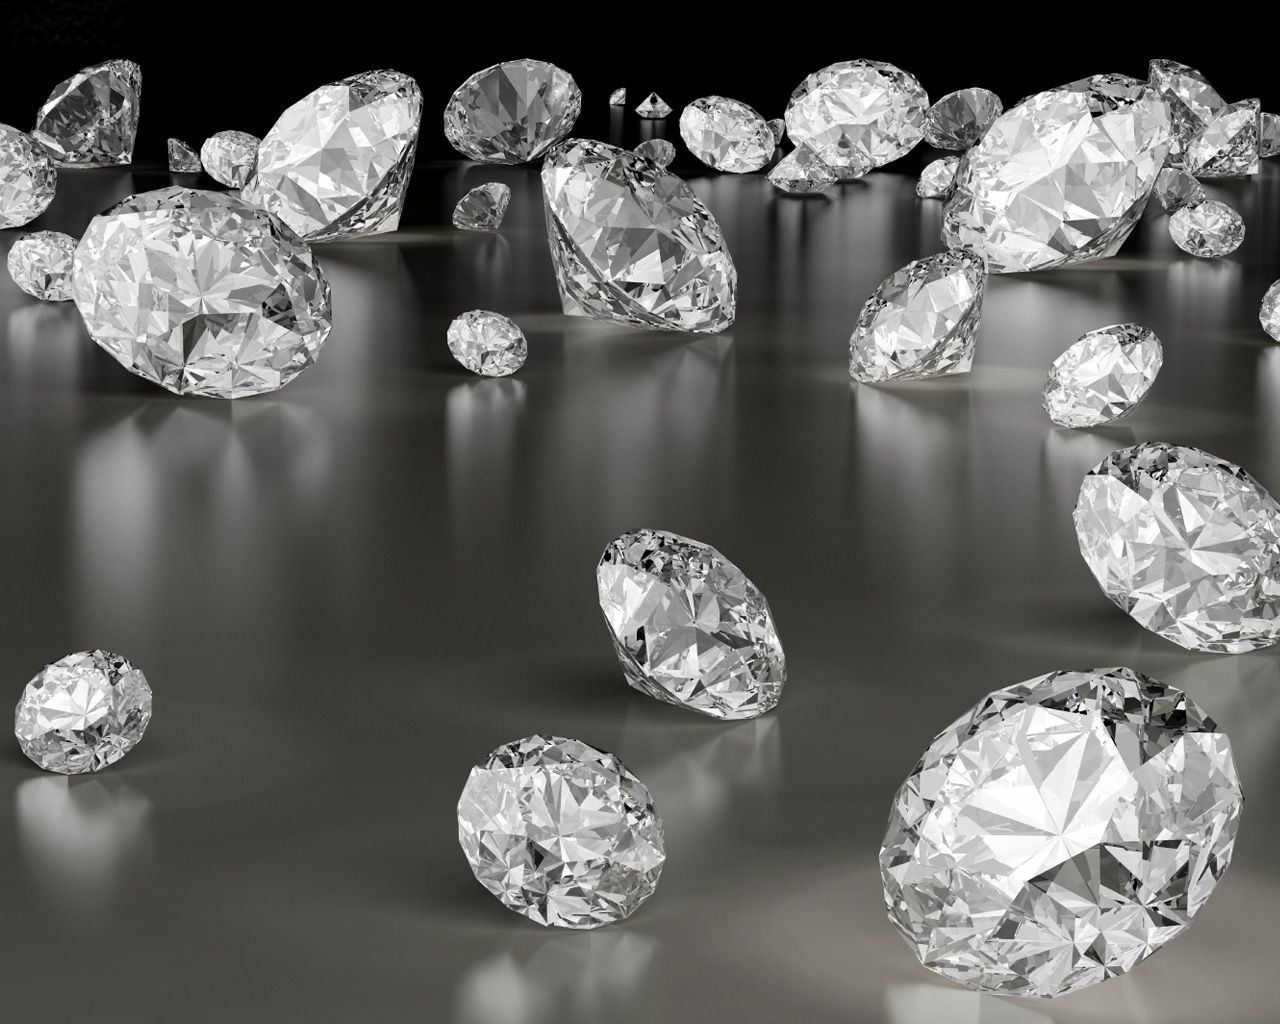
\includegraphics[height=\paperheight,width=\paperwidth]{bkg.jpg}};}
\begin{frame}
	\begin{center}
		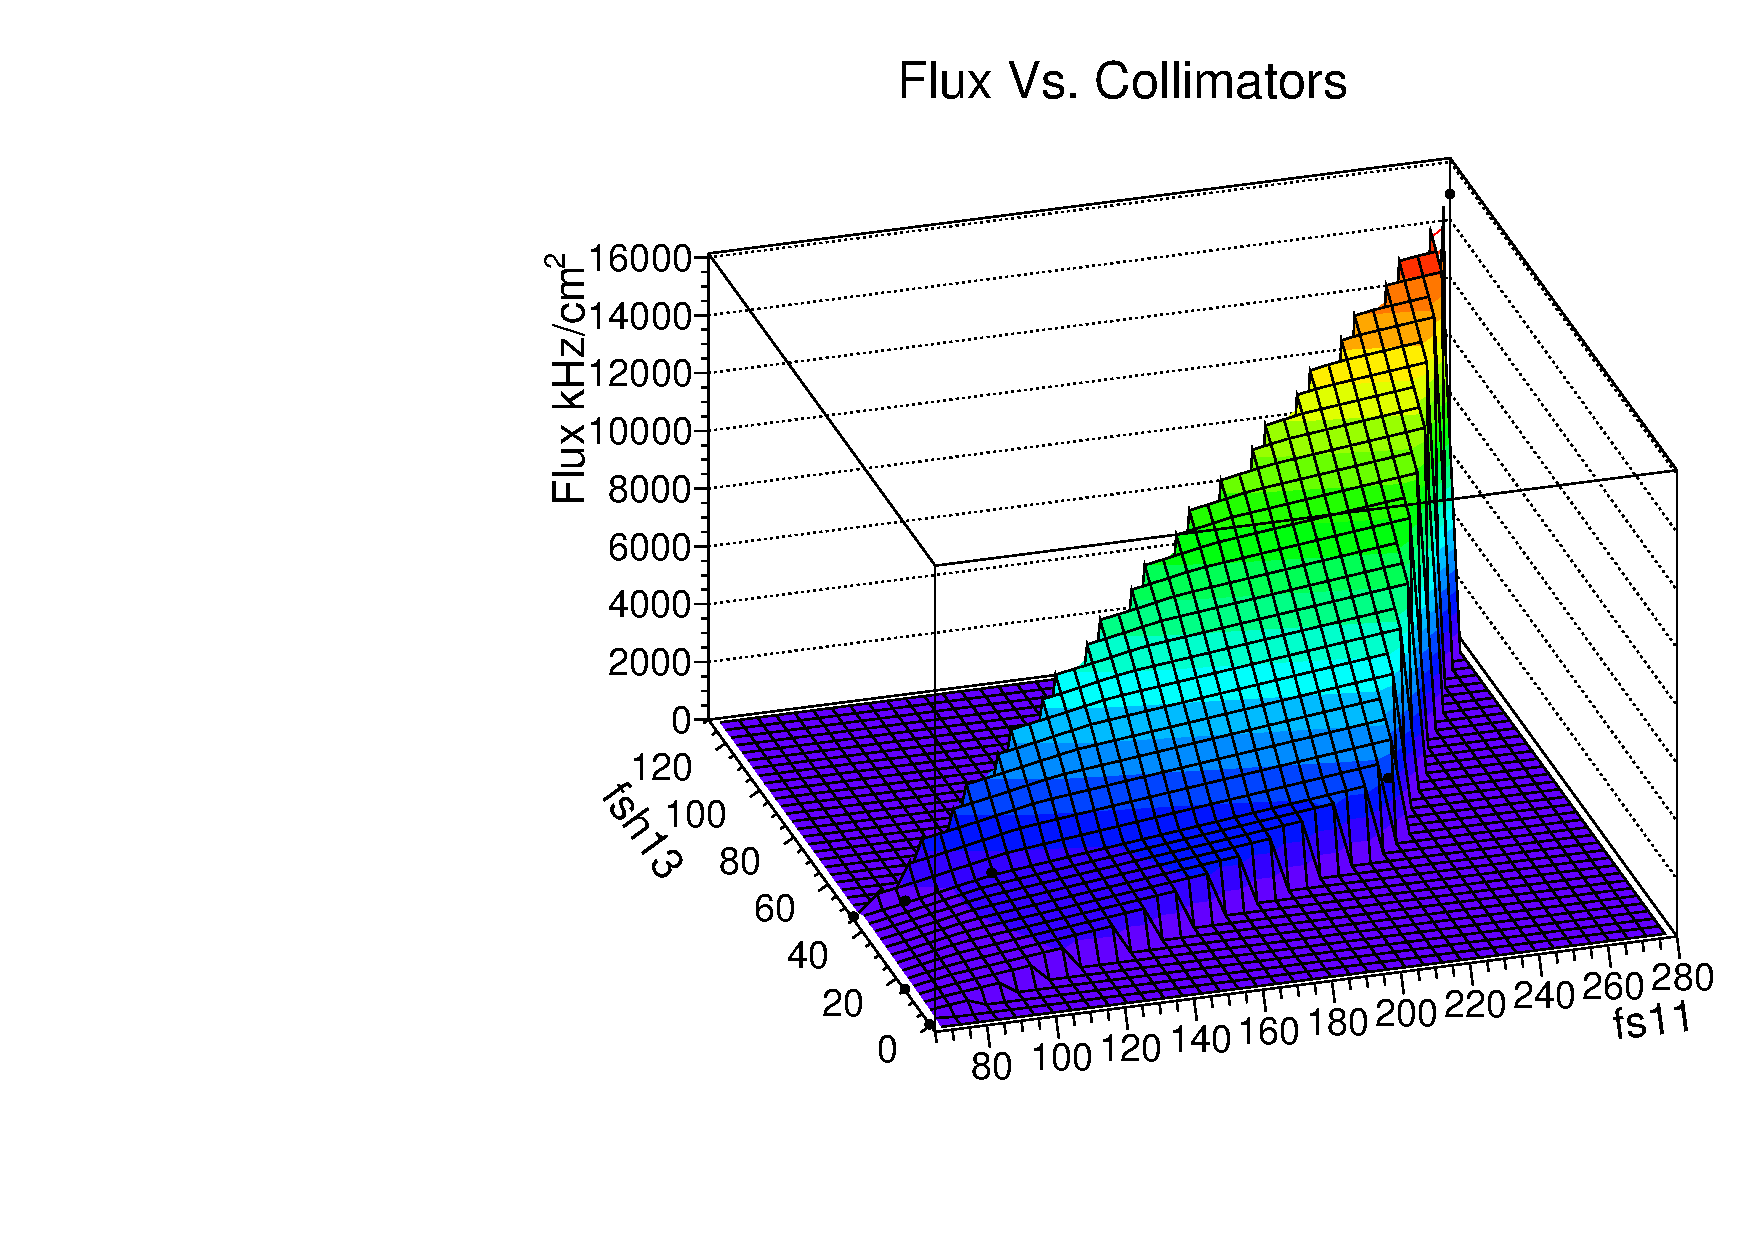
\includegraphics[angle=270, width=4cm]{FluxVsCollimators}
	\end{center}
	\begin{alertblock}{
		\begin{center}
			\textbf{Reproducibility of the Rate Settings}
		\end{center}}
		\vspace*{10pt}
		\begin{center}\small
		Speaker: Michael Reichmann
		\end{center}\normalsize
	\end{alertblock}
\end{frame}
\usebackgroundtemplate{}
% END
% ============================
% BEGIN TABLE OF CONTENTS
% ============================
\begin{frame}[allowframebreaks]
	\frametitle{Table of contents}
	\tableofcontents   % [pausesections]
\end{frame}
% END
% ====================================================================================
% BEGIN COL SETTINGS
% ====================================================================================
\section{Collimator Settings}
% ============================
\begin{frame}
	\frametitle{Collimator Settings}
	\begin{minipage}{6cm}
		\centering
		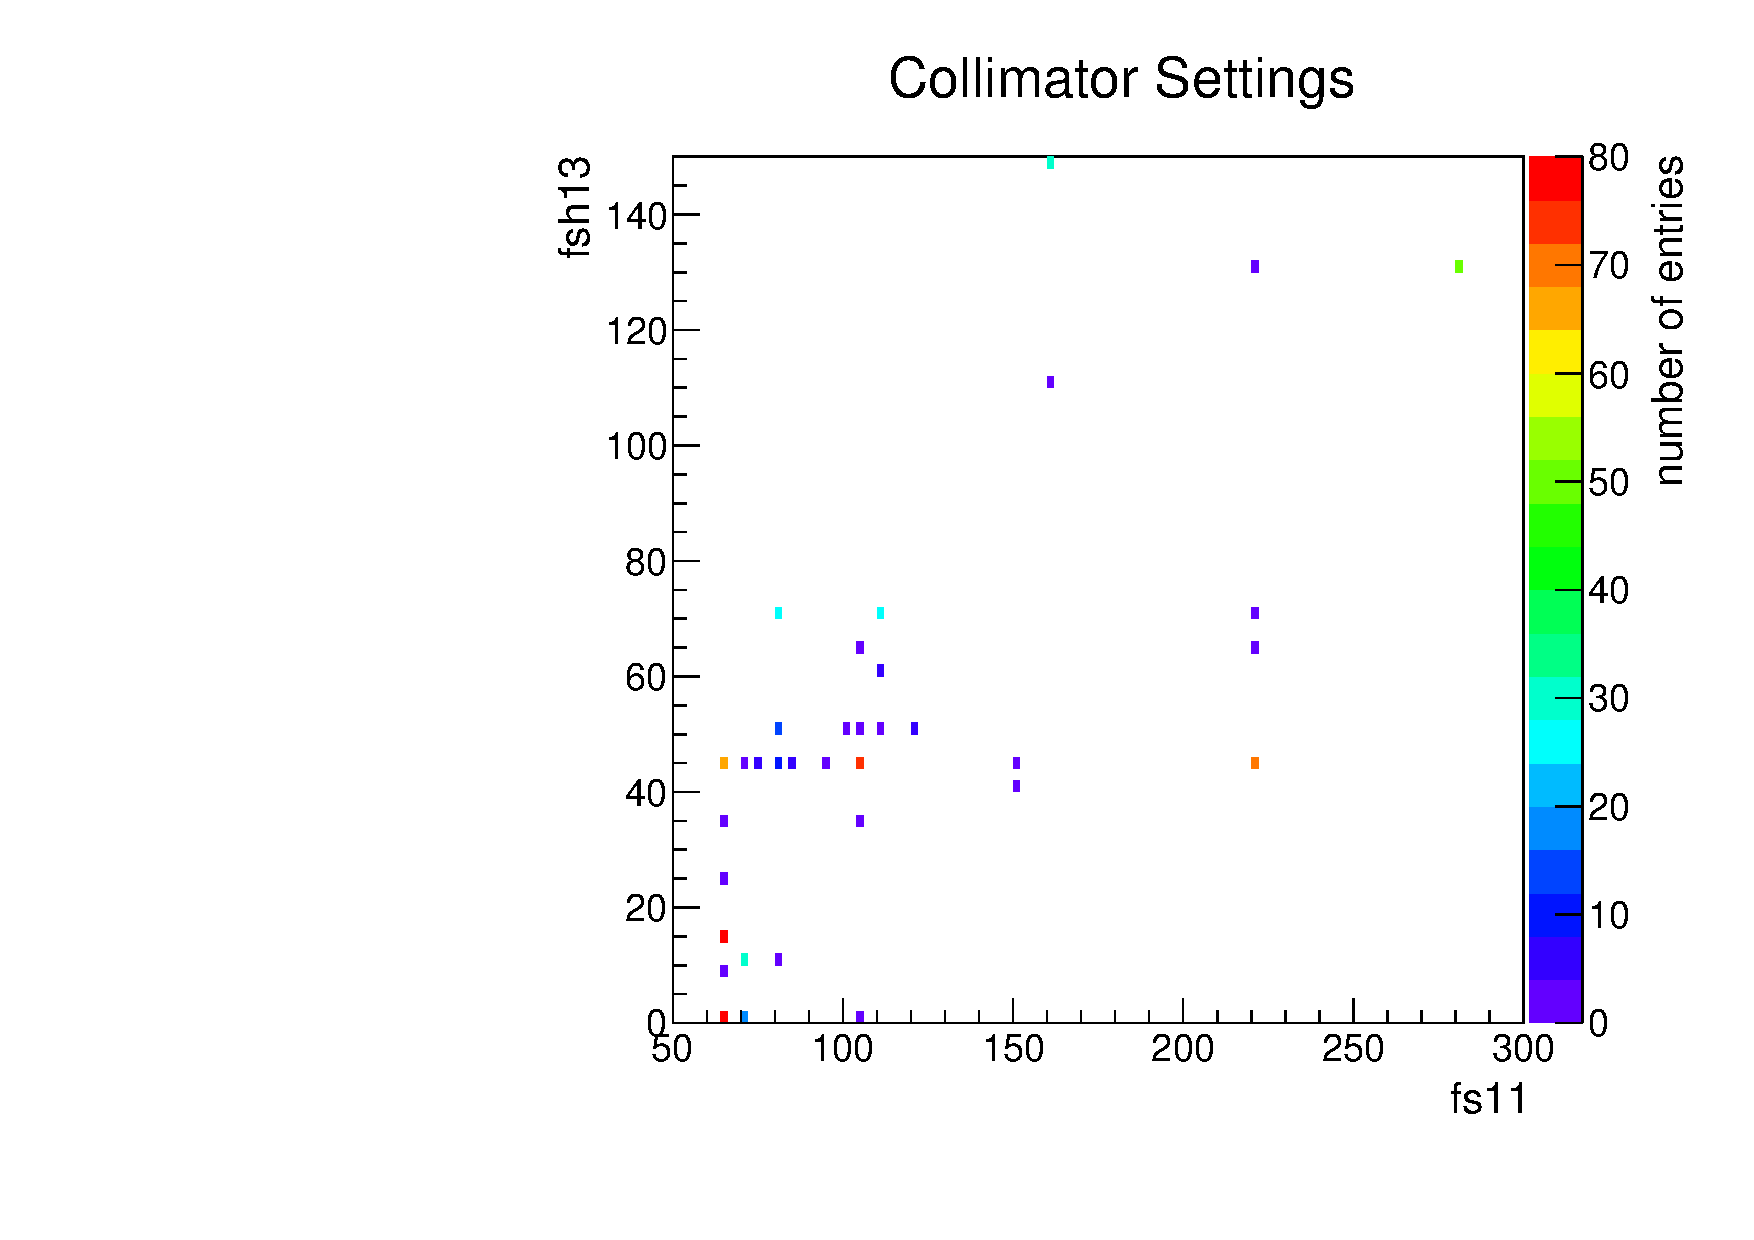
\includegraphics[angle=270, width=5cm]{CollimatorSettings}
	\end{minipage}
	\hspace*{2pt}
	\begin{minipage}{5cm}
		\begin{table}[c]
			\small
			\begin{tabular}{l|l|l}\toprule
				fs11	& fsh13	& flux [kHz/cm$^{2}$]\\\hline
				$65$	& $0.5$ & $3$\\\hline
				$65$	& $15$ & $20$\\\hline
				$65$	& $45$ & $60$\\\hline
				$105$	& $45$ & $200$\\\hline
				$220$	& $45$ & $2000$\\\hline
				$280$	& $130$ & $500$\\
				\bottomrule
			\end{tabular}
			\caption{aimed fluxes for the collimator settings in Aug/Oct 2015}
		\end{table}
	\end{minipage}
	\begin{itemize}
		\item plot shows all settings we ever saved in May/Aug/Oct 2015
		\item collimators:
		\begin{itemize}
			\item fs11: in front of first bending magnet,
			\item fsh13: in the intermediate focus point between the two bending magnet
		\end{itemize}
		\item reddish and green points are the settings we chose for the rate scans in Aug/Oct 2015
	\end{itemize}
\end{frame}
% new frame ============================
\begin{frame}
	\frametitle{Beam Area}
	\begin{center}
		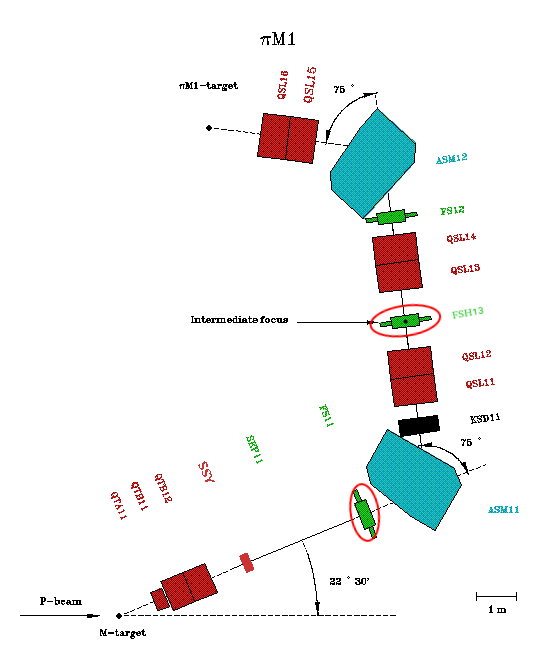
\includegraphics[height=7.5cm]{pim1}
	\end{center}
\end{frame}
% new frame ============================
\begin{frame}
	\begin{center}
		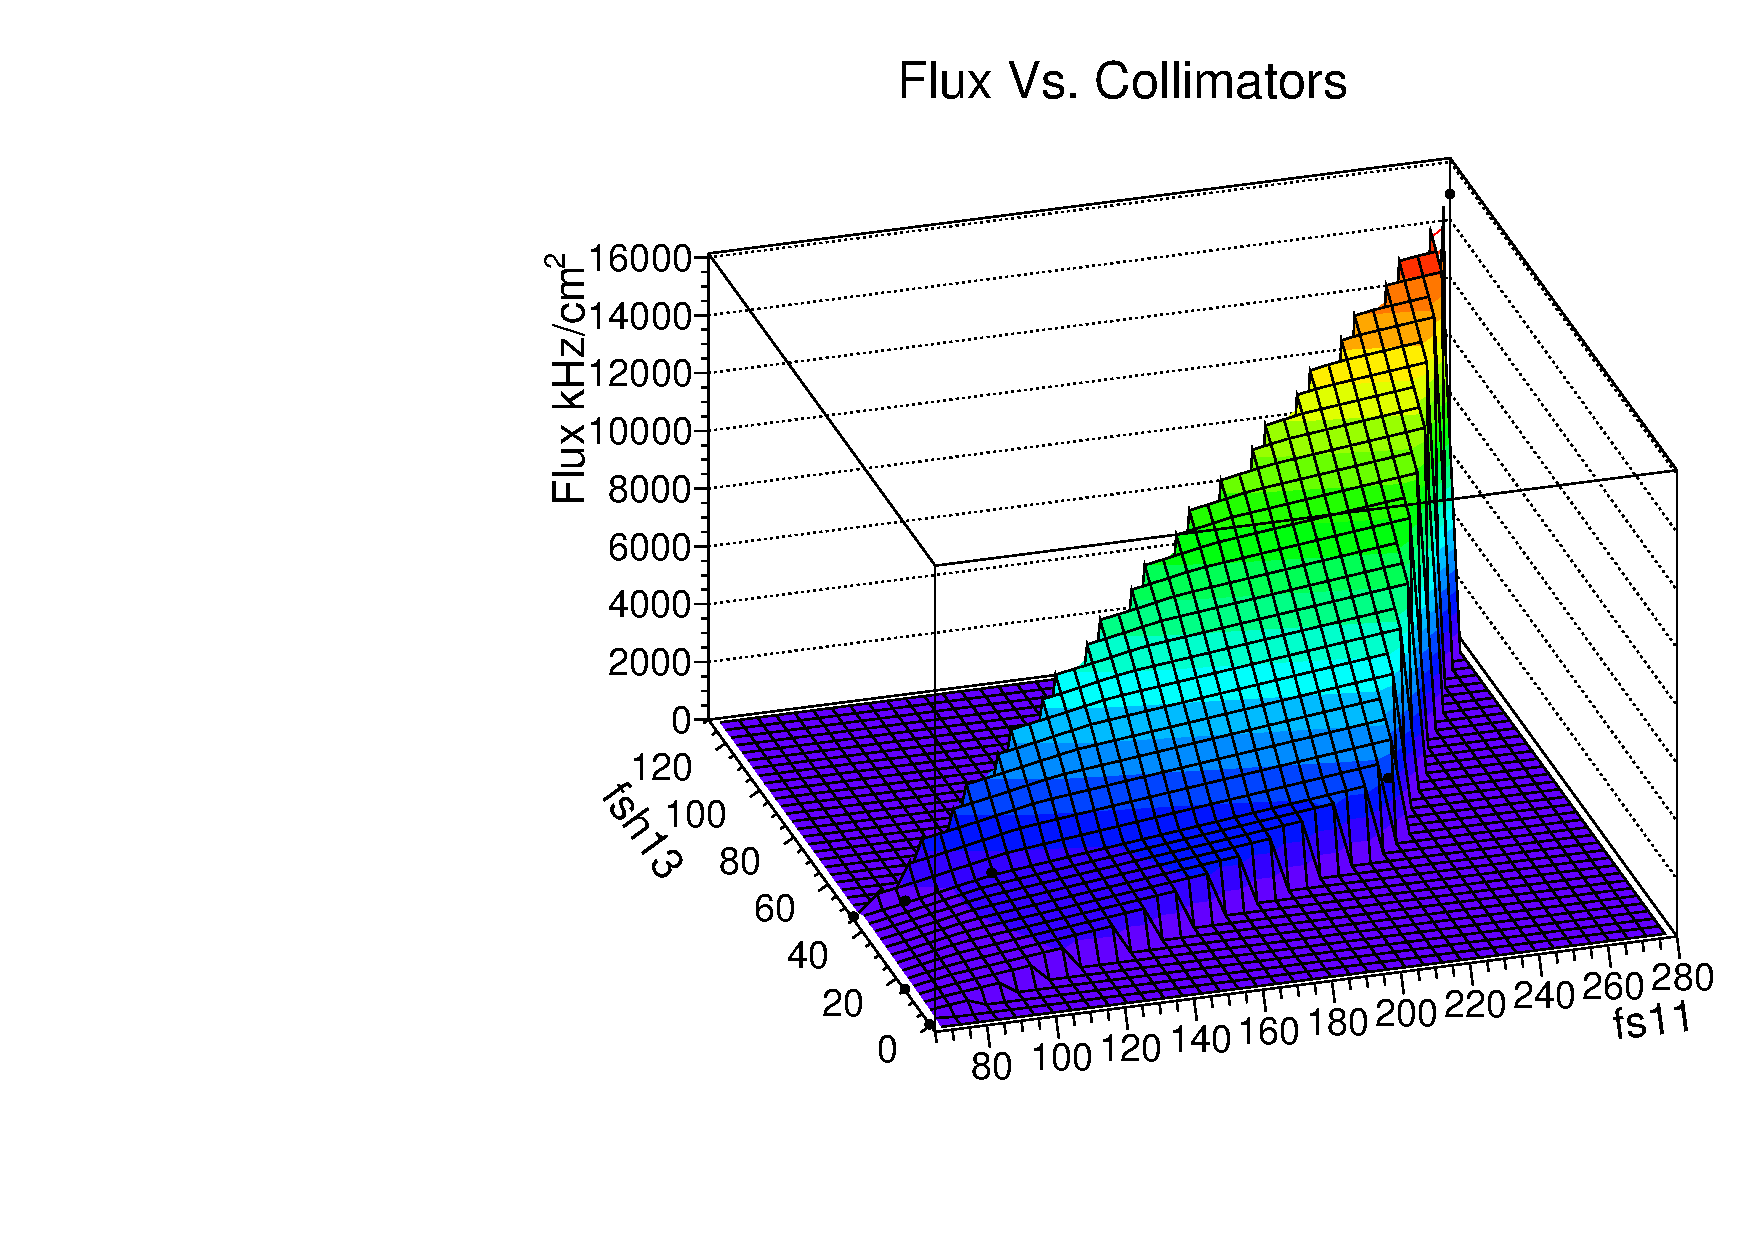
\includegraphics[angle=270, width=8cm]{FluxVsCollimators}
	\end{center}
\end{frame}
% ============================
% END
% ====================================================================================
% BEGIN FLUX STABILITY
% ====================================================================================
\section{Stability of the Flux}
% ============================
\begin{frame}
	\frametitle{Flux Distributions for all runs}
	\begin{minipage}{3.5cm}
		\centering
		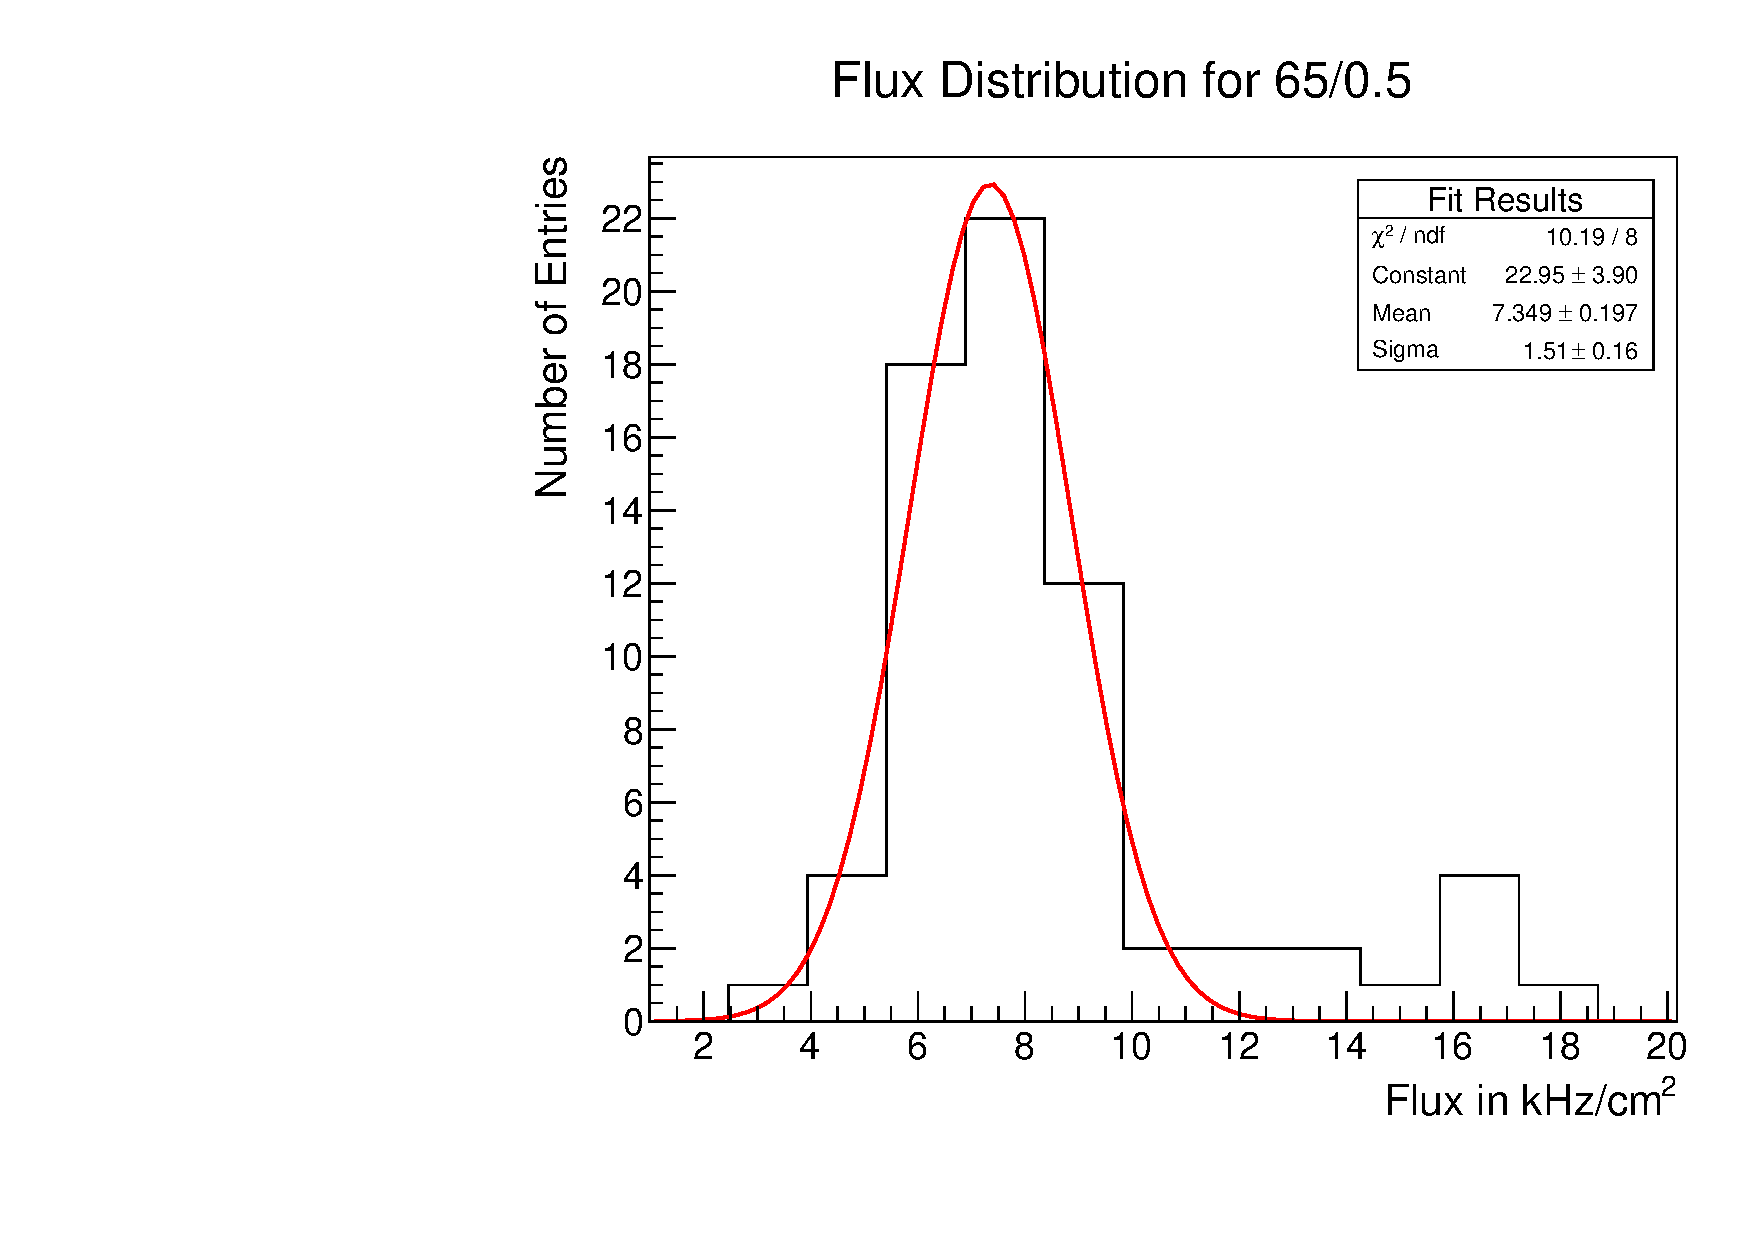
\includegraphics[angle=270, width=3.5cm]{FluxDistribution65_0}
	\end{minipage}
	\hspace*{2pt}
	\begin{minipage}{3.5cm}
		\centering
		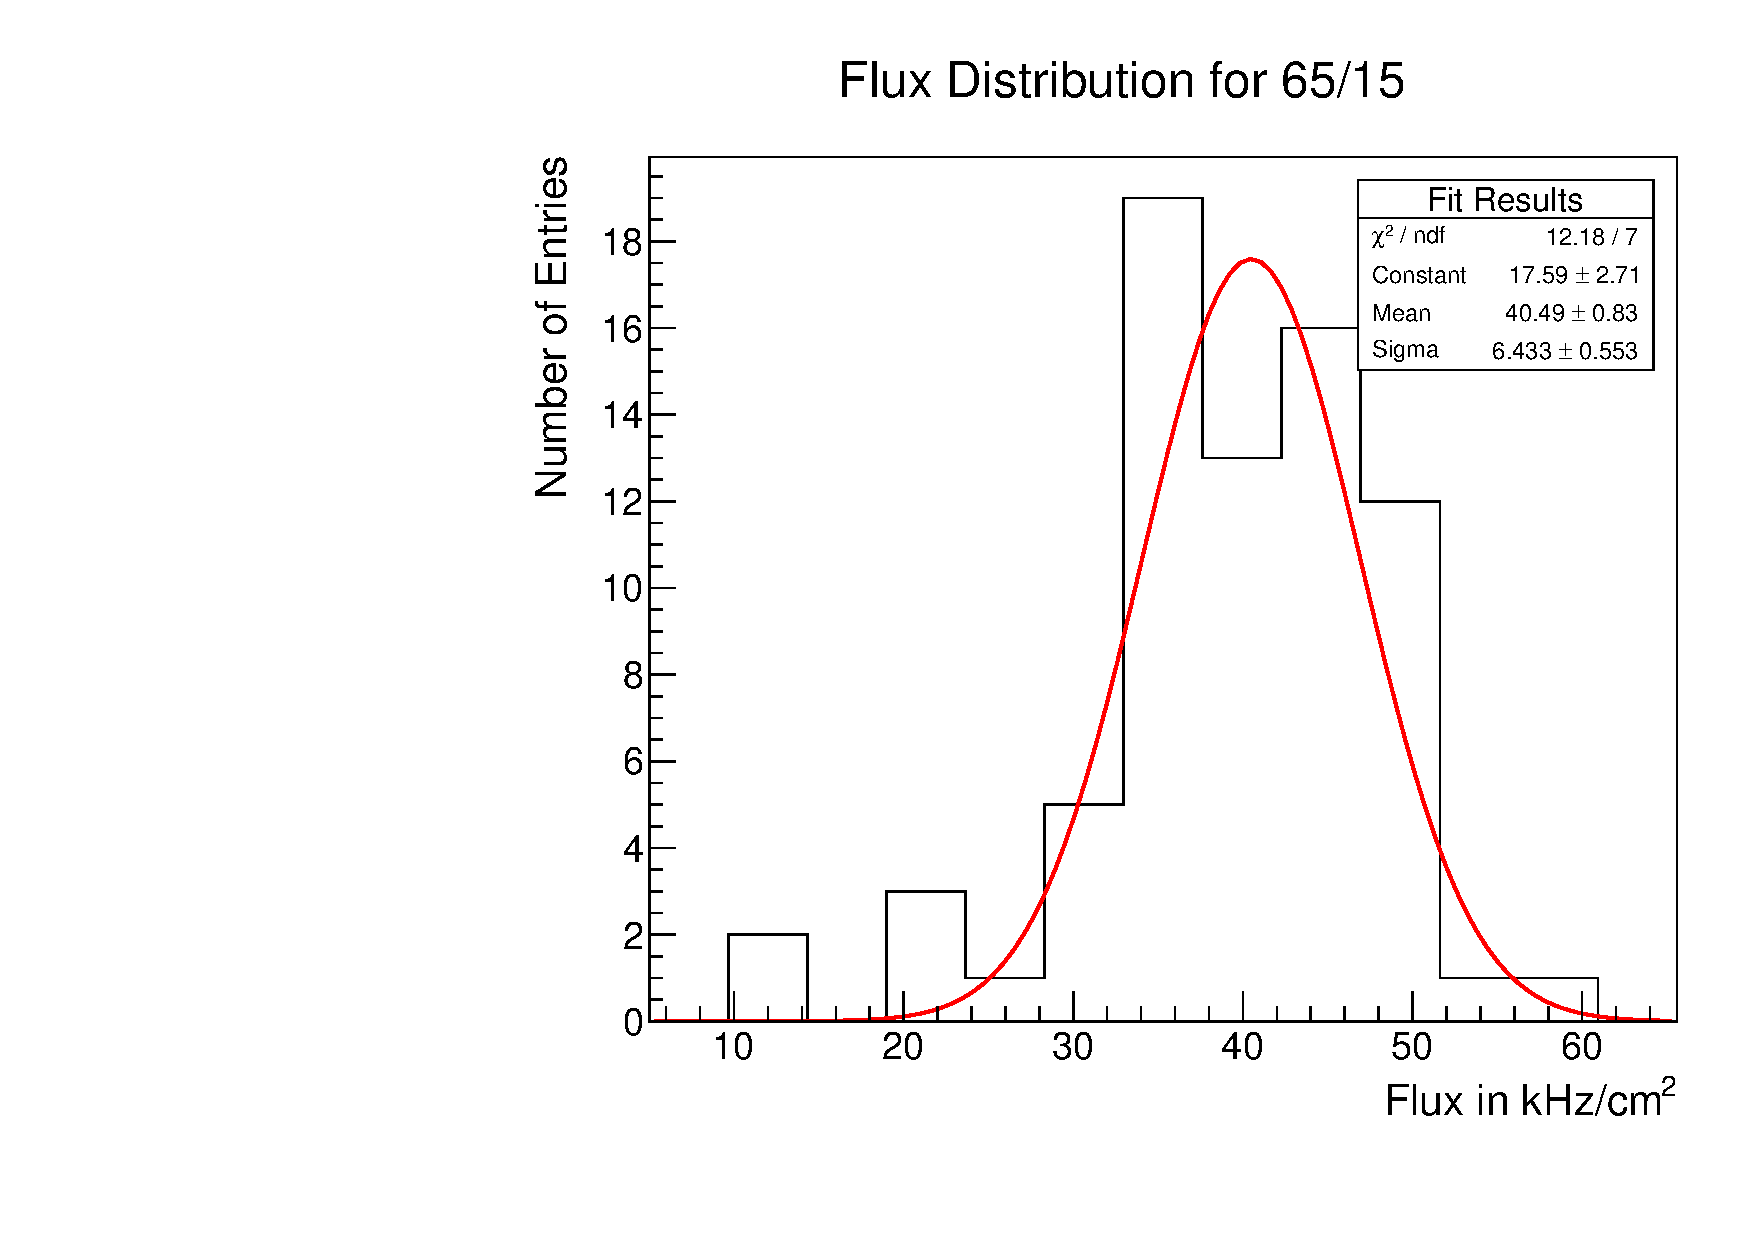
\includegraphics[angle=270, width=3.5cm]{FluxDistribution65_15}
	\end{minipage}
	\hspace*{2pt}
	\begin{minipage}{3.5cm}
		\centering
		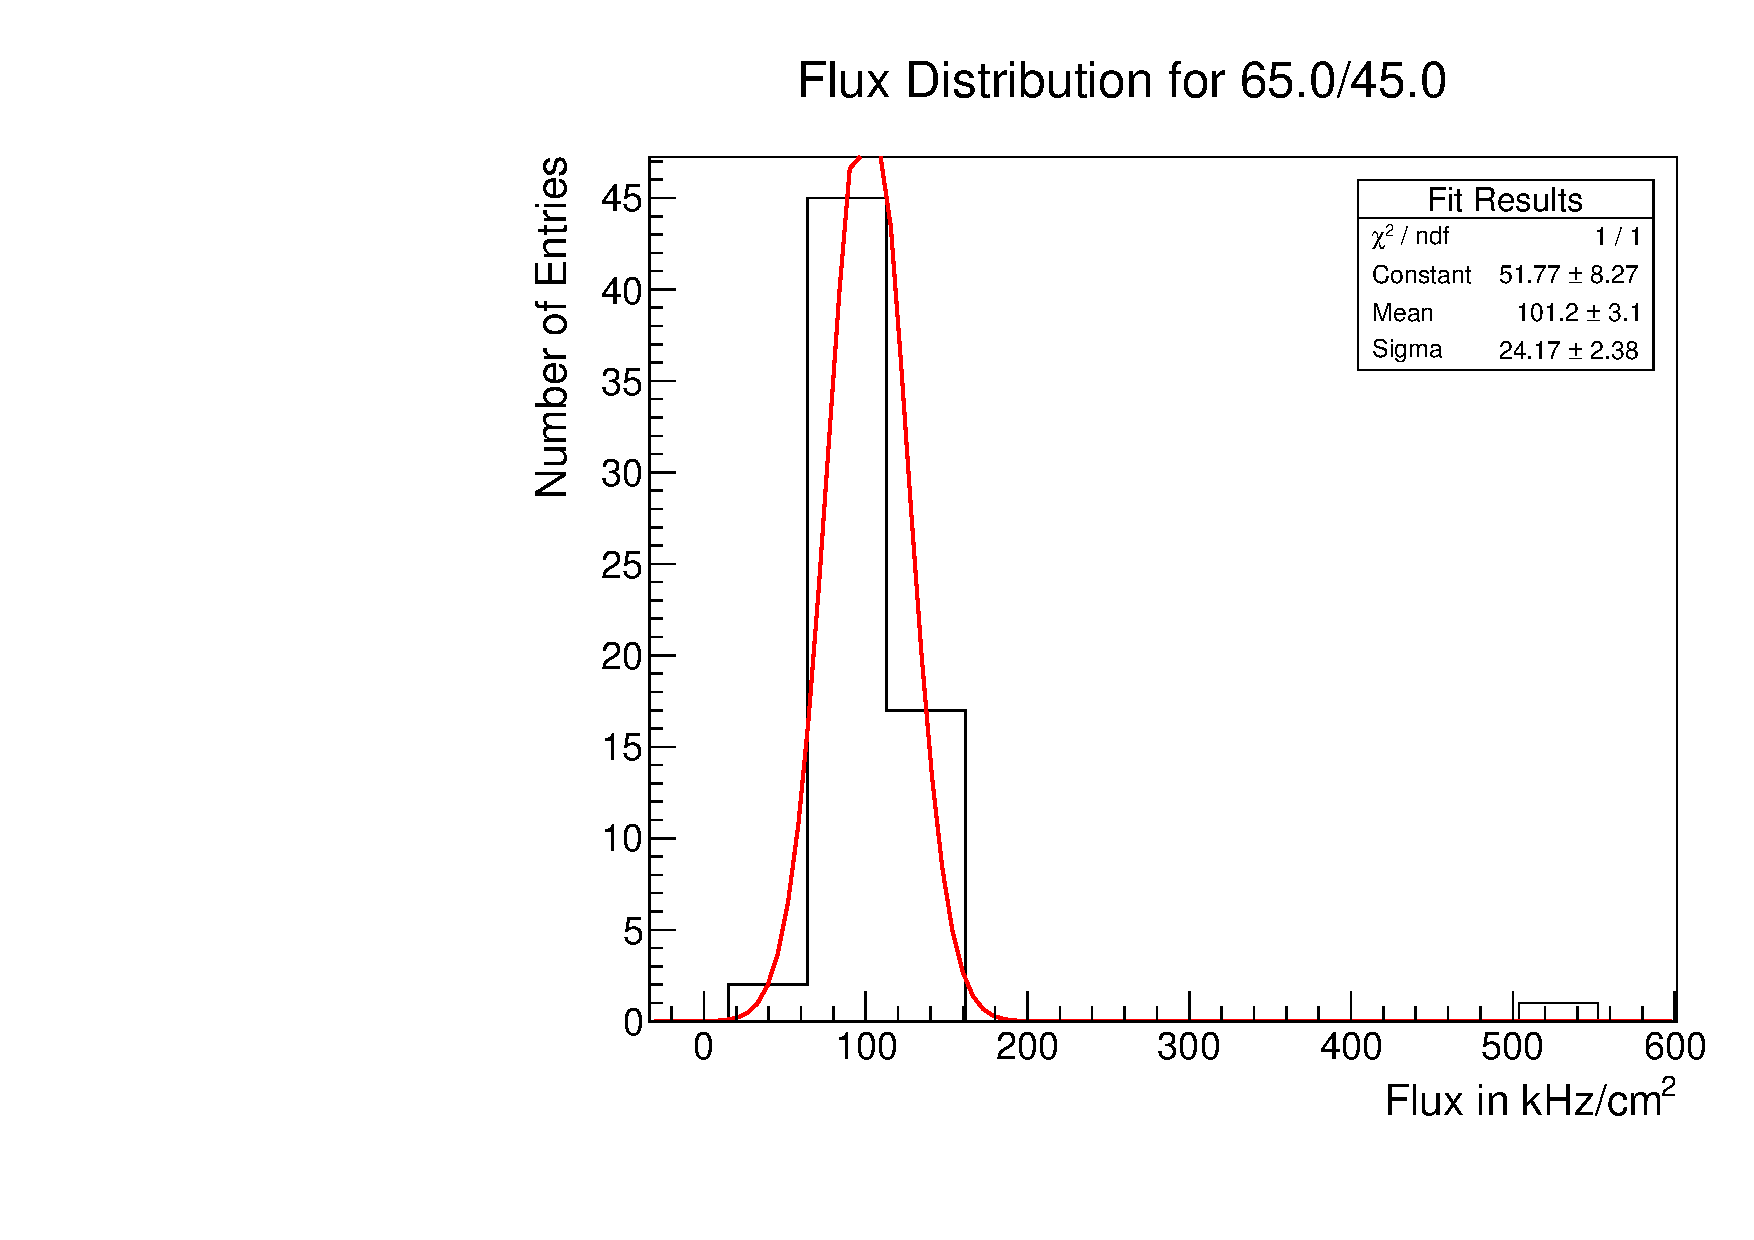
\includegraphics[angle=270, width=3.5cm]{FluxDistribution65_45}
	\end{minipage}\s
	\begin{minipage}{3.5cm}
		\centering
		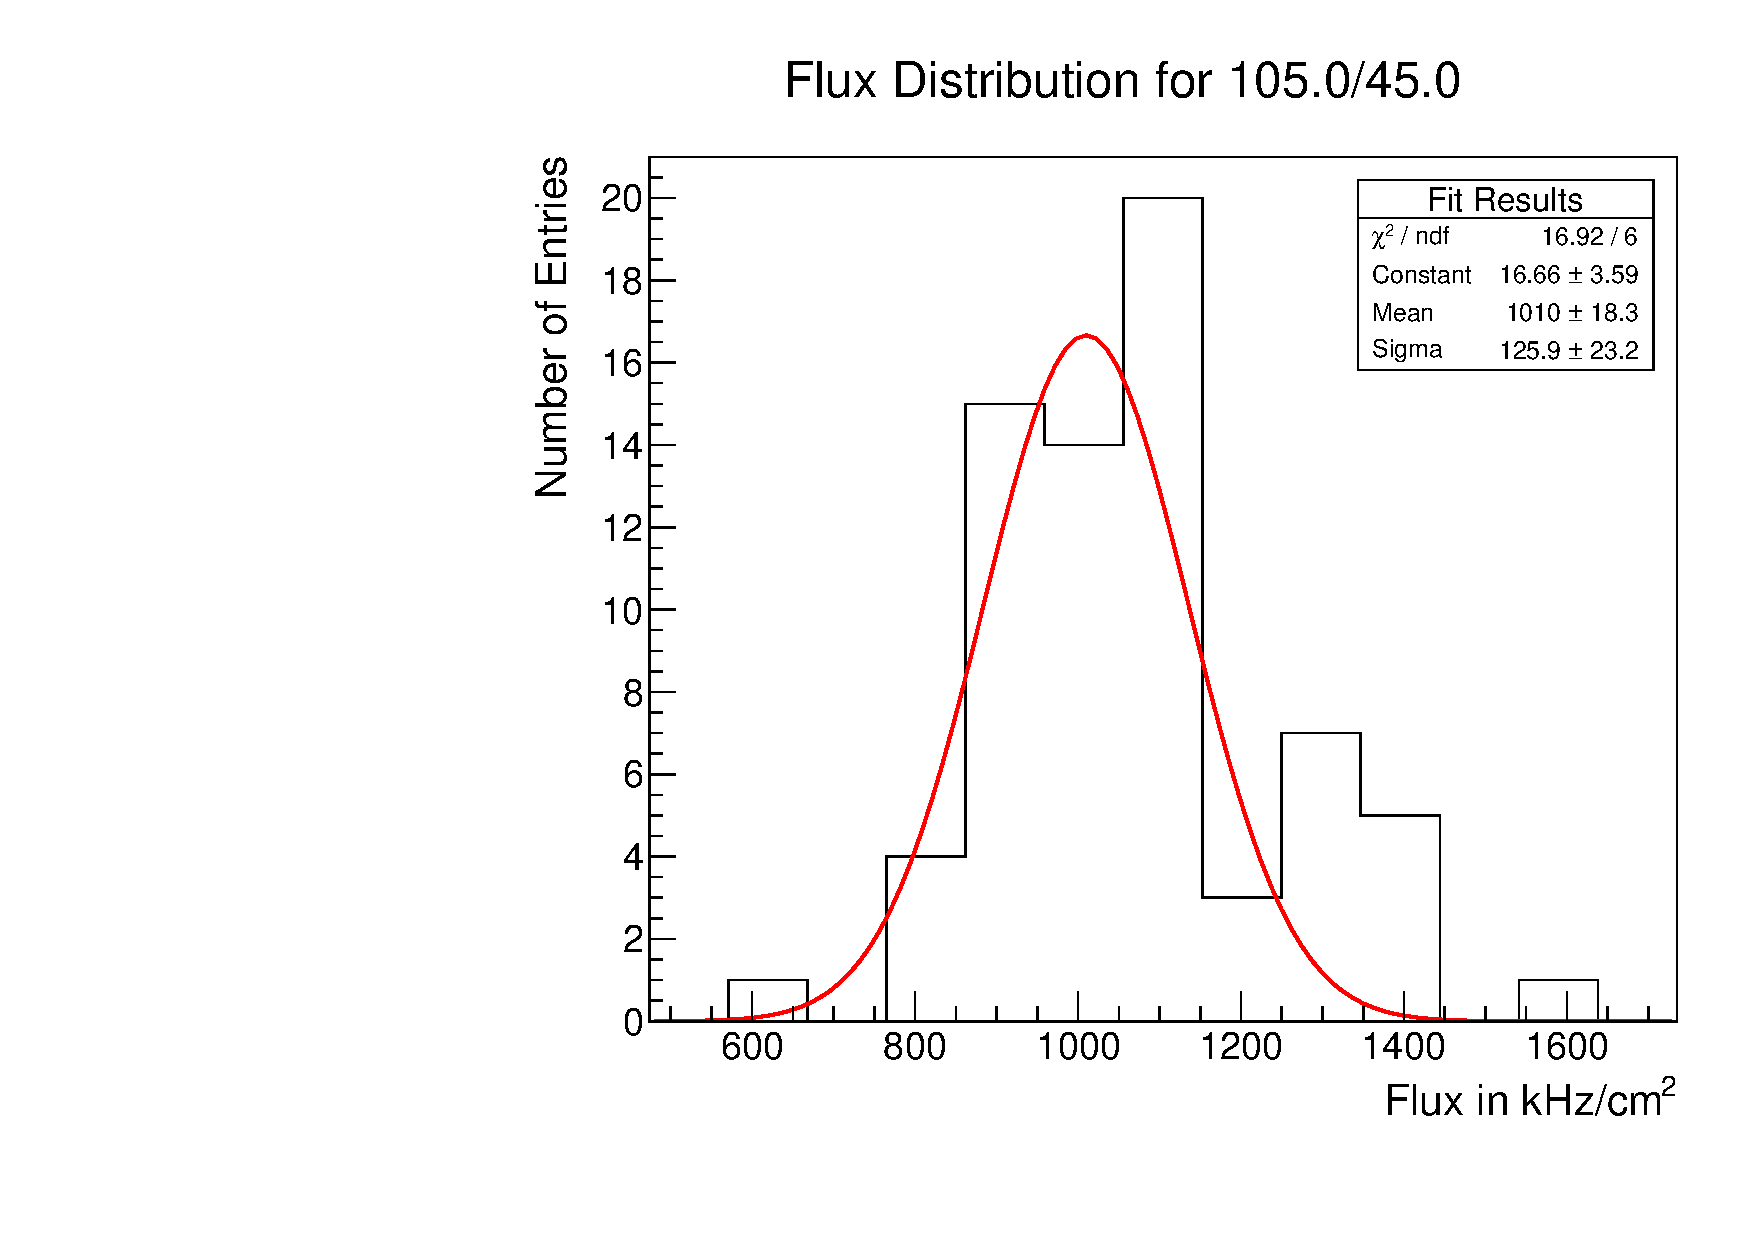
\includegraphics[angle=270, width=3.5cm]{FluxDistribution105_45}
	\end{minipage}
	\hspace*{2pt}
	\begin{minipage}{3.5cm}
		\centering
		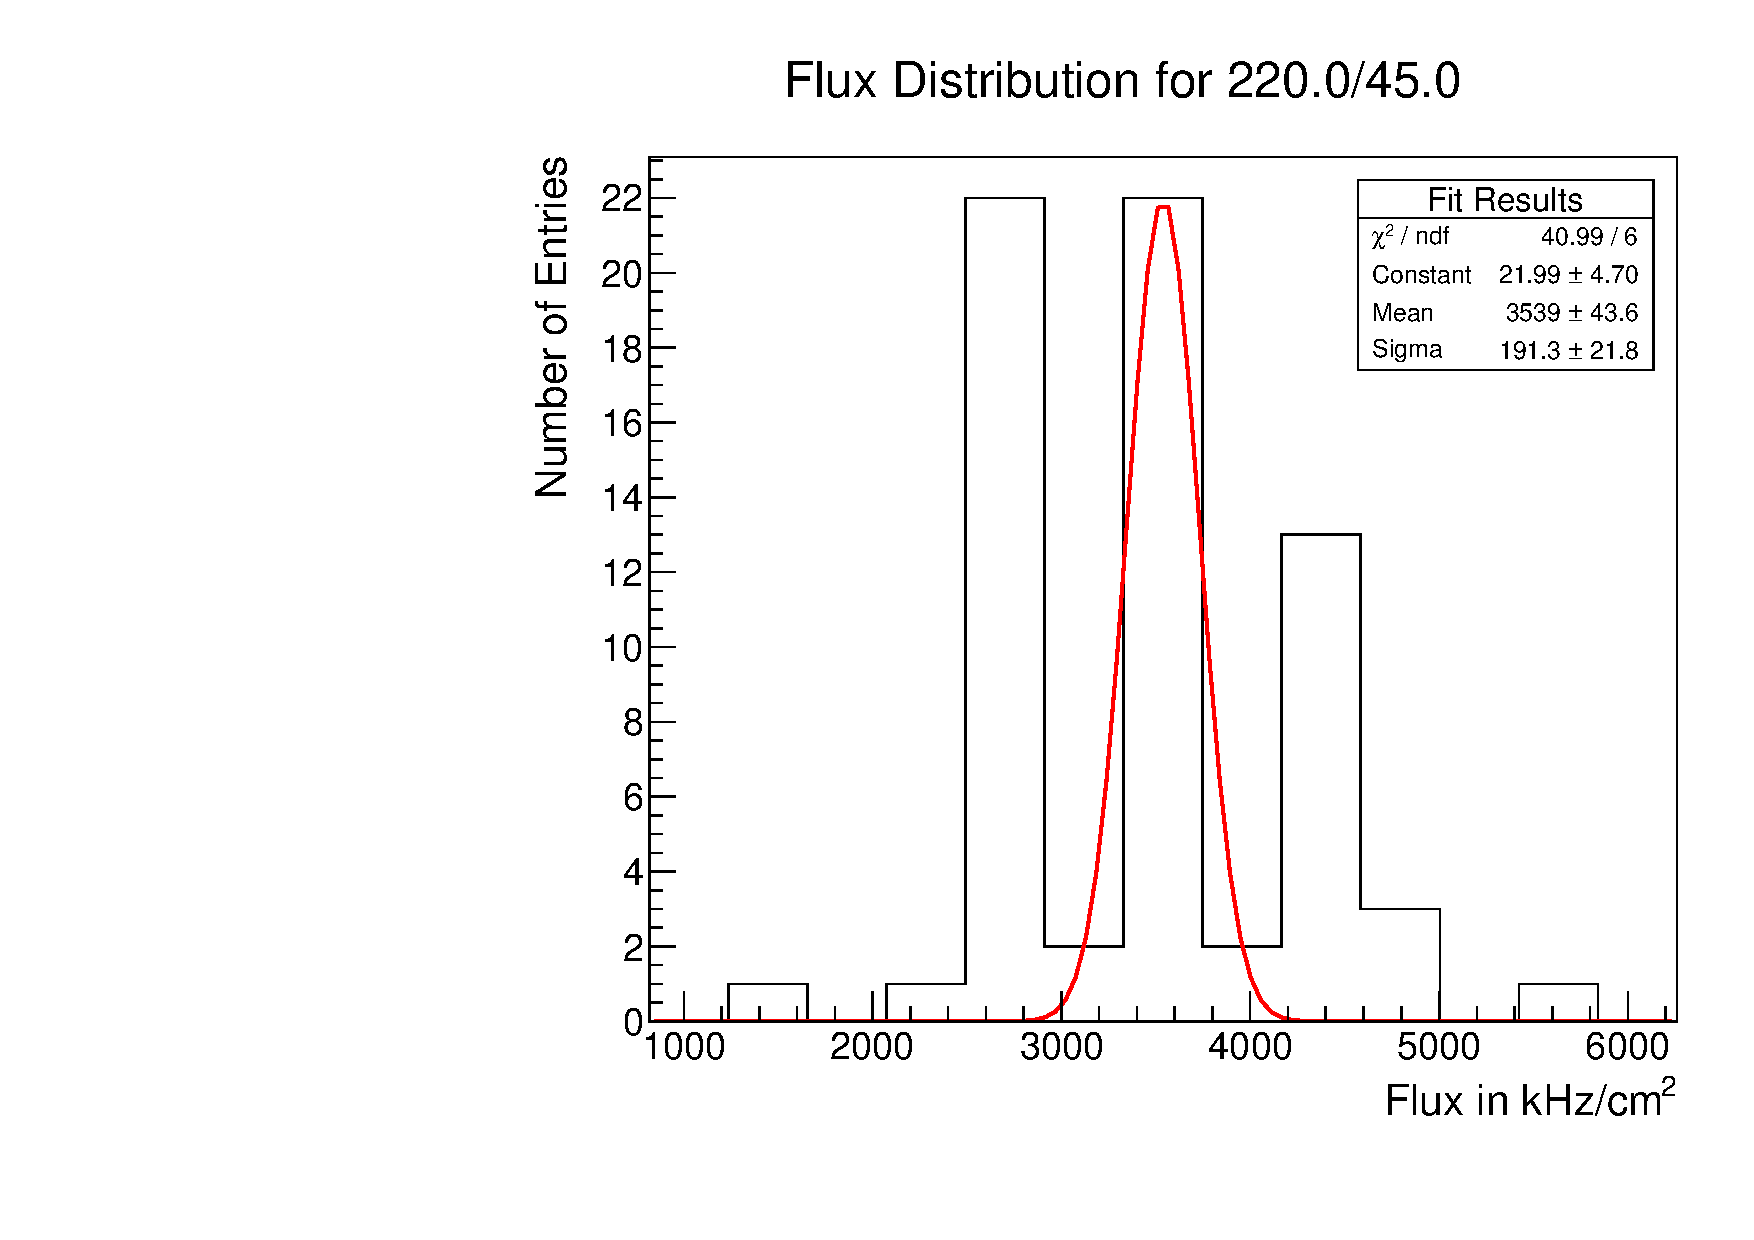
\includegraphics[angle=270, width=3.5cm]{FluxDistribution220_45}
	\end{minipage}
	\hspace*{2pt}
	\begin{minipage}{3.5cm}
		\centering
		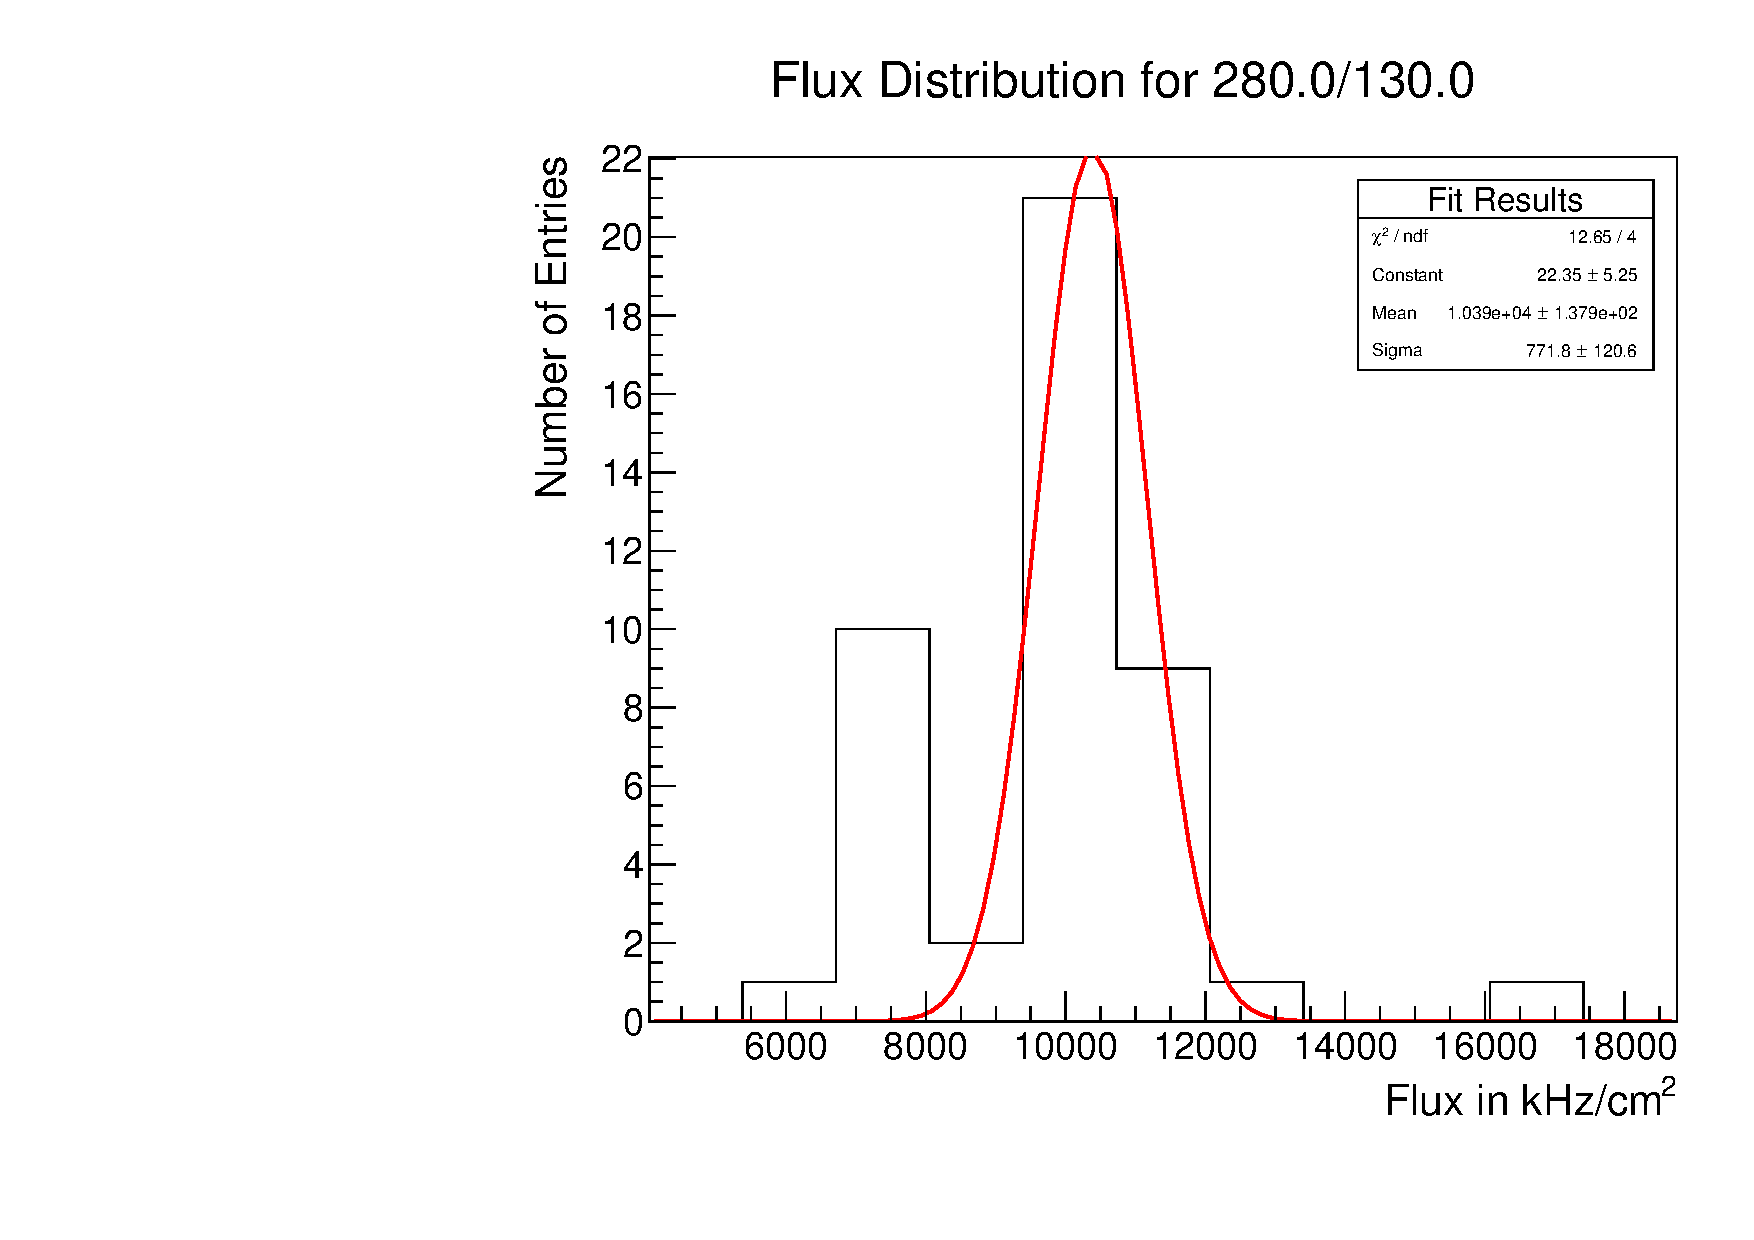
\includegraphics[angle=270, width=3.5cm]{FluxDistribution280_130}
	\end{minipage}\s
\end{frame}
% new frame ============================
\begin{frame}
	\frametitle{Flux Deviations}
	\begin{minipage}{5.5cm}
		\centering
		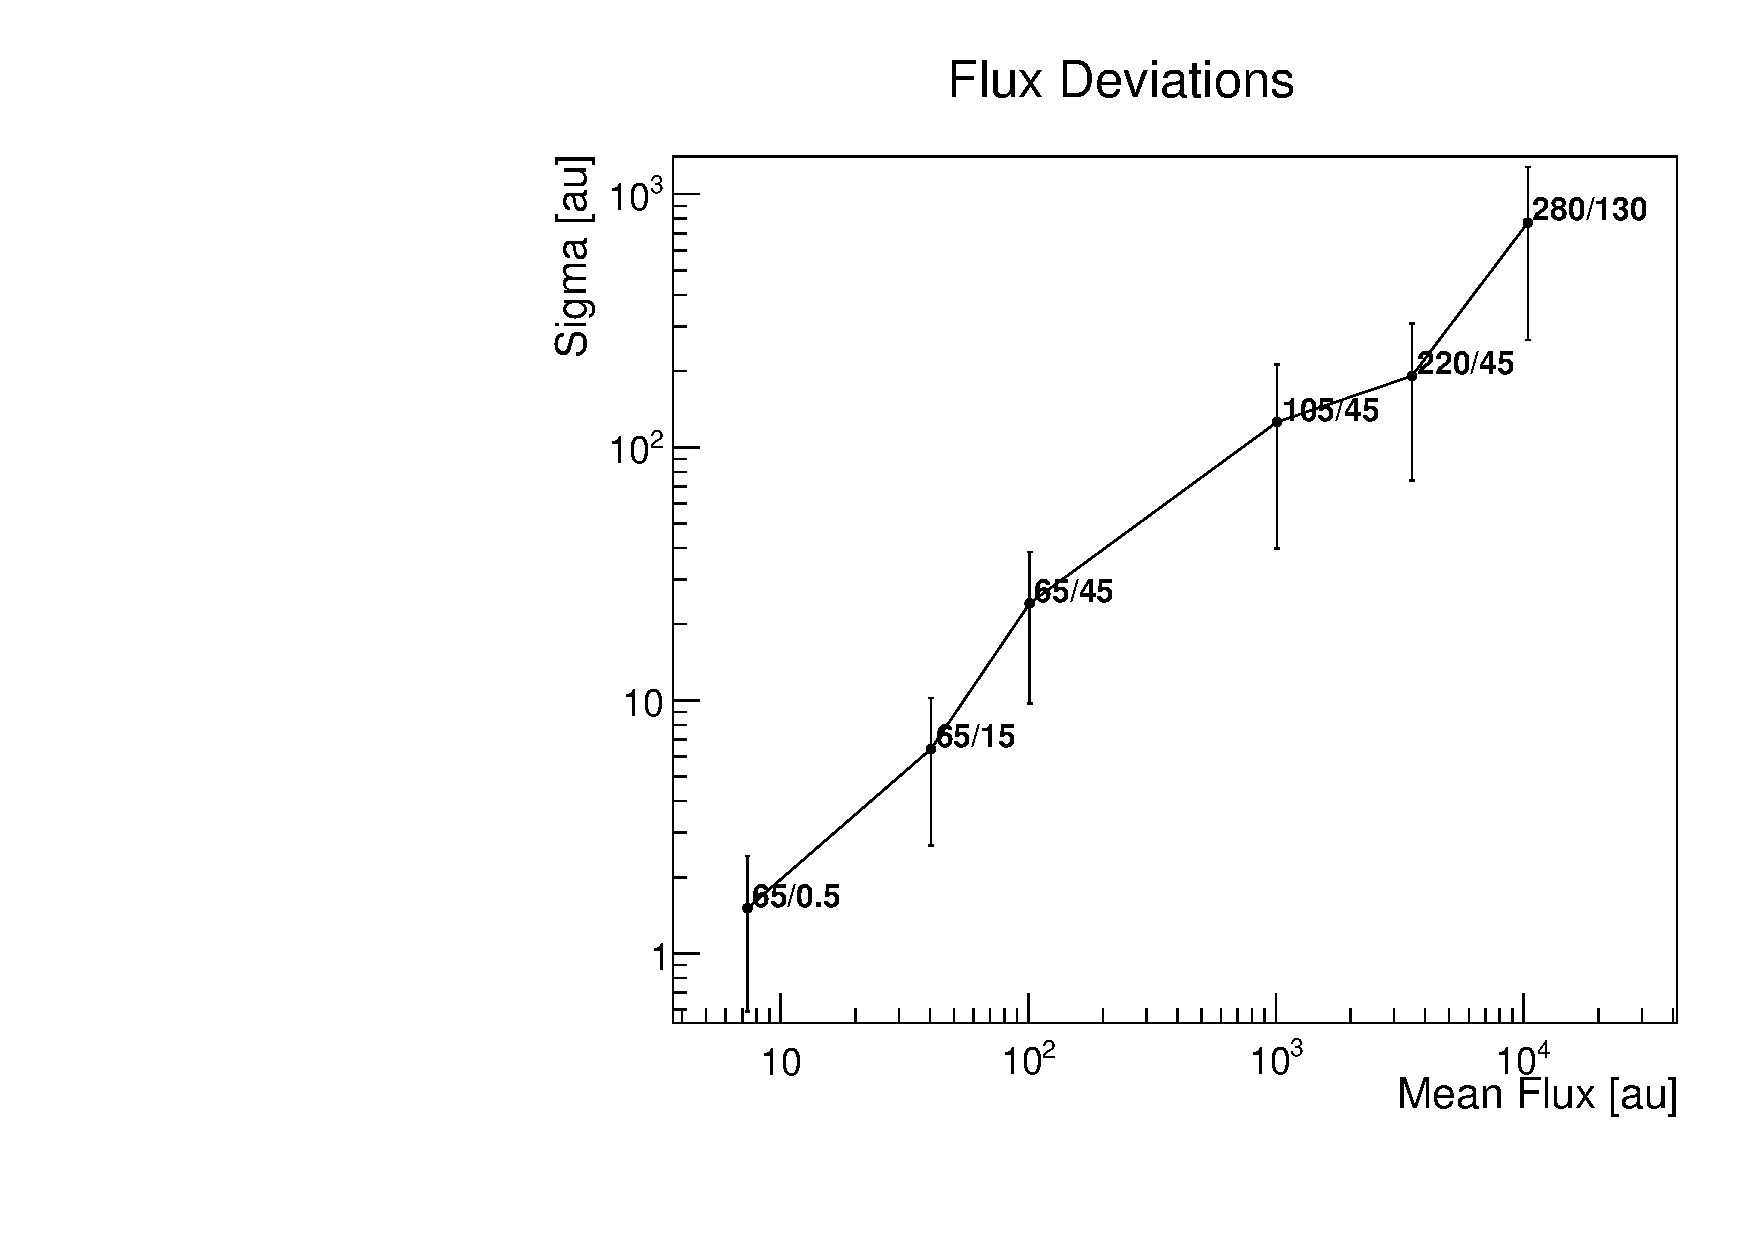
\includegraphics[angle=270, width=5.5cm]{FluxVariations}
	\end{minipage}
	\hspace*{2pt}
	\begin{minipage}{5.5cm}
		\centering
		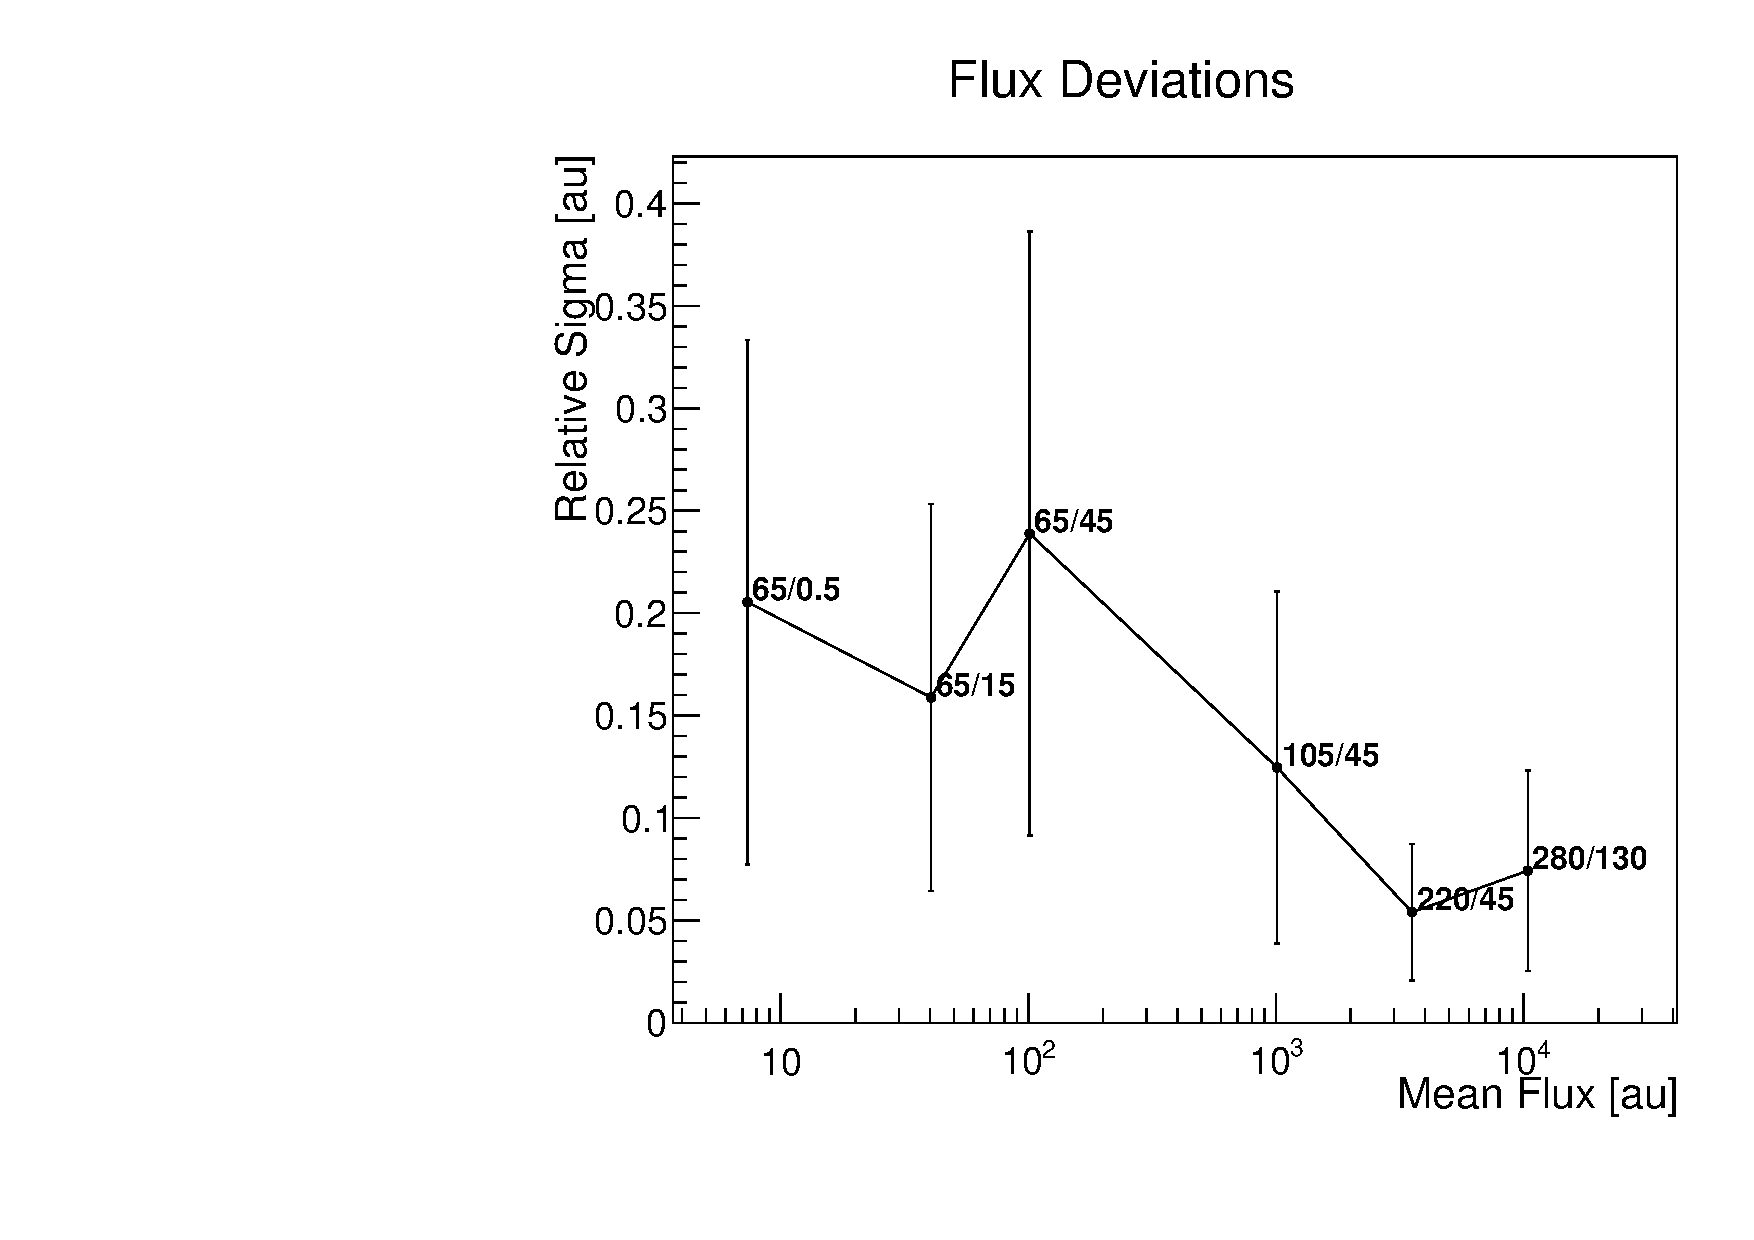
\includegraphics[angle=270, width=5.5cm]{FluxVariationsRel}
	\end{minipage}
	\begin{itemize}
		\item huge error bars due to uncertainties caused by:
		\begin{itemize}
			\item wrongly entered fast-OR rates (beam stop, typos)
			\item inconsistencies of different setups
			\item different mask sizes (Gaussian beam profile)
		\end{itemize}
	\end{itemize}
\end{frame}
% new frame ============================
\begin{frame}
	\frametitle{Fluxes Within One Rate Scan}
	\begin{table}[t]
		\footnotesize
		\begin{tabular}{c|c|c|c|c|c|c|c}
			\toprule
			\textbf{FS11/FSH13}	& \textbf{65/0.5}	& \textbf{65/15}	& \textbf{65/45}	& \textbf{80/45}	& \textbf{105/45}	& \textbf{220/45}	& \textbf{280/130}\\\hline
					& 13.6	& 44.5	& 107.6	& 392.1	& 1114.5	& 3335.7	& 10090.3\\
					& 14.1	& 44.6	& 107.6	& 406.6	& 1093.6	& 3366.3	& 10146.8\\
					& 14.8	& 45.0	& 108.2	& 392.5	& 1117.3	& 3364.9	& 10235.6\\
					& 15.8	& 44.9	& 107.9	& 411.0	& 1100.8	& 3359.3	& \\
					& 		& 45.3	& 108.5	& 395.6	& 1123.5	& 3380.2	& \\
					& 		& 46.1	& 109.8	& 		& 1108.2	& 3376.5	& \\\hline
			Mean	& 14.6	& 45.1	& 108.3	& 399.6	& 1109.6	& 3363.8	& 10157.6\\
			Sigma	& 0.8	& 0.5	& 0.8	& 7.8	& 10.1		& 14.4		& 59.8\\
			\bottomrule
		\end{tabular}
		\caption{RunPlan 8 in October 2015 (II6-B2 and poly-D @ \SI{-1000}{V})}
	\end{table}
	\vspace*{-10pt}
	\begin{table}[t]
		\footnotesize
		\begin{tabular}{c|c|c|c|c|c|c|c}
			\toprule
			\textbf{FS11/FSH13}	& \textbf{65/0.5}	& \textbf{65/15}	& \textbf{65/45}	& \textbf{80/45}	& \textbf{105/45}	& \textbf{220/45}	& \textbf{280/130}\\\hline
					& 16.7	& 47.1	& 110.9	& 411.5	& 1131.3	& 3405.8	& 10190.0\\
					& 16.1	& 46.2	& 105.6	& 399.5	& 1109.2	& 3395.9	& 10180.3\\
					& 16.8	& 46.9	& 110.3	& 416.8	& 1139.4	& 3420.6	& {\color{red}6143.1}\\
					& 17.4	& 46.8	& 111.2	& 400.6	& 1122.3	& 3423.8	& \\
					& 		& 47.5	& 110.5	& 417.1	& {\color{red}1000.9}	& 3444.1	& \\
					& 		& 47.9	& 110.8	& 403.9	& 1125.9	& 3444.6	& \\\hline
			Mean	& 16.8	& 47.1	& 109.9	& 408.2	& 1104.8	& 3422.5	& 8837.8\\
			Sigma	& 0.5	& 0.5	& 1.9	& 7.3	& 47.4		& 18.0		& 1905.4\\
			\bottomrule
		\end{tabular}
		\caption{RunPlan 10 in October 2015 (II6-B2 and poly-D @ \SI{1000}{V})}
	\end{table}
\end{frame}
% ============================
% END
% ====================================================================================
% BEGIN CONCLUSION
% ====================================================================================
\section{Conclusion}
% ============================
\begin{frame}
	\frametitle{Conclusion}
	\begin{minipage}[c][.3\textheight]{\textwidth}
		\begin{itemize}
			\setlength{\itemsep}{\fill}
			\item fluxes during a single rate scan are very stable and reproducible within a couple percent
			\item fluxes for different setup may very within the order of \SI{10}{\%}
			\item with the new setup the rates are saved automatically during the whole run $\longrightarrow$ more accurate measurement
		\end{itemize}
	\end{minipage}
\end{frame}
% END
% DOCUMENT END
\end{document}

